% Provenance (never printed): see sources/outline_sources.md (Year 2: metamorphic reactions,
% Clapeyron slopes, the Al2SiO5 diagram, the facies grid, protoliths). Definitions and facies
% table from the IUGS subcommission proposal (via the Granada translation); thermodynamic data
% from Robie and Hemingway (1995); experimental diagram from Holdaway and Mukhopadhyay (1993);
% curves from figdata/bachelor-2/facies.py; exercise and problem values in the Book 4 scratch
% calculator calc/ch10.py.
\chapter{Réactions métamorphiques et faciès}\label{ch:b2:metamorphic-facies}

Un basalte qui plonge avec sa plaque ne reste pas un basalte. Son plagioclase et son pyroxène
réagissent à l'état solide pour donner d'autres minéraux, et le nouvel assemblage dépend de la
pression et de la température atteintes~: une roche bleue de glaucophane et de lawsonite, ou une
roche verte et rouge d'omphacite et de grenat. Les roches métamorphiques conservent ces minéraux lorsqu'elles
remontent à la surface, et un pétrologue qui connaît les réactions peut en lire les
conditions. Ce chapitre écrit ces réactions avec la thermodynamique vue dans le volume de chimie, calcule à partir de données mesurées
le diagramme de phases métamorphique le plus célèbre, celui des trois
minéraux \ce{Al2SiO5}, le compare à l'expérience,
et organise les assemblages des roches métamorphiques en faciès.
% ledger: scmr:facies-assemblages

\begin{recall}
\textbf{Du volume de lycée}~: \omterm{def:b2:metamorphic-facies:metamorphism}{métamorphisme}, degré métamorphique, minéraux indicateurs
et isogrades, \omterm{def:b2:metamorphic-facies:metamorphism}{métamorphisme} de contact et son auréole, foliation et schistosité,
pression lithostatique~; disthène, andalousite et sillimanite comme polymorphes, et leur
diagramme de phases. \textbf{Des volumes de physique et de chimie de première année}~: l'énergie de Gibbs
$G = H - TS$, dont le minimum marque l'état stable à $T$ et $P$ donnés~;
enthalpie, entropie et capacité thermique~; $\mathrm dG = V\,\mathrm dP - S\,\mathrm dT$~; la
relation de Clausius--Clapeyron pour la vaporisation d'un corps pur et le point
triple de l'eau. \textbf{Du volume de première année}~: zones de subduction, chaînes de collision et
le géotherme.
\end{recall}

\section{Métamorphisme}\label{sec:b2:metamorphic-facies:metamorphism}

Le volume de lycée abordait le \omterm{def:b2:metamorphic-facies:metamorphism}{métamorphisme} comme la transformation d'une roche par la chaleur et
la pression. Une recommandation internationale donne la définition retenue ici.

\begin{definition}[Métamorphisme~; protolithe]\label{def:b2:metamorphic-facies:metamorphism}
\emph{Métamorphisme}\index{métamorphisme} est un processus qui modifie les minéraux ou la
microstructure d'une roche, ou les deux, essentiellement à l'état solide, lorsque la roche s'ajuste
à des conditions physiques différentes de celles dans lesquelles elle s'est formée et de celles
qui règnent normalement à la surface de la Terre et dans la zone de diagenèse. Il peut coexister avec
une \omterm{def:b2:mantle-melting:melting}{fusion partielle} et modifier la composition chimique de la roche. La roche avant
son métamorphisme est son \emph{protolithe}\index{protolithe}.
\end{definition}
% ledger: scmr:metamorphism

La limite inférieure exclut la diagenèse, les transformations d'un sédiment enfoui puis
lithifié, et la limite supérieure est la fusion, étudiée au \cref{ch:b2:crustal-melting}. Les
agents sont la température, la pression, les fluides qui circulent dans la roche (eau et
dioxyde de carbone surtout) et la déformation. Le \omterm{def:b2:metamorphic-facies:metamorphism}{métamorphisme} se classe selon son étendue et
son cadre.
% ledger: scmr:metamorphism, scmr:types

Le \omterm{def:b2:metamorphic-facies:metamorphism}{métamorphisme} \emph{régional} touche de grands volumes de roche et accompagne de grands
processus tectoniques~: il est \emph{orogénique} dans les chaînes de montagnes, où la croûte s'épaissit lors d'une
collision~; le \omterm{def:b2:metamorphic-facies:metamorphism}{métamorphisme} d'\emph{enfouissement} touche des roches profondément enfouies sous
des empilements sédimentaires ou volcaniques épais, sans déformation ni magmatisme, de sorte que ses roches
manquent en général de schistosité~; le \omterm{def:b2:metamorphic-facies:metamorphism}{métamorphisme} \emph{océanique} modifie la croûte près des
dorsales, où l'eau de mer chaude circule à travers elle sous de forts gradients thermiques,
et sa recristallisation reste en général incomplète. Le \omterm{def:b2:metamorphic-facies:metamorphism}{métamorphisme} \emph{local}
a une cause locale~: le \omterm{def:b2:metamorphic-facies:metamorphism}{métamorphisme} \emph{de contact} chauffe les roches encaissantes d'une intrusion~;
le \omterm{def:b2:metamorphic-facies:metamorphism}{métamorphisme} \emph{hydrothermal} est lié à des fluides chauds riches en eau~;
le \omterm{def:b2:metamorphic-facies:metamorphism}{métamorphisme} \emph{de dislocation}, dans les zones de faille et de cisaillement, réduit la taille des grains et
produit des mylonites et des cataclasites~; le \omterm{def:b2:metamorphic-facies:metamorphism}{métamorphisme} \emph{d'impact}, sous l'effet d'une
\omterm{def:b2:planet-formation-meteorites:fall-find}{météorite}, peut fondre et vaporiser la roche. Le \omterm{def:b2:metamorphic-facies:metamorphism}{métamorphisme} est dit prograde tant que la
température monte, et rétrograde tant qu'elle baisse.
% ledger: scmr:types

\section{Réactions métamorphiques}\label{sec:b2:metamorphic-facies:reactions}

\begin{definition}[Réaction métamorphique~; réaction de dévolatilisation]\label{def:b2:metamorphic-facies:reaction}
Une \emph{réaction métamorphique}\index{réaction métamorphique} transforme un ensemble de minéraux
d'une roche, les réactifs, en un autre ensemble, les produits, à l'état solide,
éventuellement avec une phase fluide qui y prend part. Une \emph{réaction de dévolatilisation}\index{réaction de dévolatilisation}
est une réaction qui libère un \omterm{def:b2:elements-in-the-earth:volatility}{élément volatil}~: de l'eau dans une réaction de
déshydratation, ou du dioxyde de carbone dans une réaction de décarbonatation.
\end{definition}

Trois types apparaîtront dans ce chapitre. Les changements polymorphiques, comme le passage du disthène
à la sillimanite ou de la calcite à l'aragonite, gardent la formule et changent la structure.
D'autres réactions entre solides redistribuent des constituants entre minéraux, comme celle où l'albite
donne de la jadéite et du quartz~:
\[
\ce{NaAlSi3O8 -> NaAlSi2O6 + SiO2}.
\]
Les \omterm{def:b2:metamorphic-facies:reaction}{réactions de dévolatilisation} libèrent un fluide, comme la décomposition de la muscovite et du quartz
à haute température~:
\[
\ce{KAl3Si3O10(OH)2 + SiO2 -> KAlSi3O8 + Al2SiO5 + H2O}.
\]
% ledger: day73:ms-qz

Pour une réaction entre minéraux de composition fixe, la variation d'énergie de Gibbs est
$\Delta_r G(T, P) = \sum G_{\text{produits}} - \sum G_{\text{réactifs}}$~; les produits
sont stables là où $\Delta_r G < 0$, les réactifs là où $\Delta_r G > 0$, et les deux
coexistent là où $\Delta_r G = 0$.

\begin{definition}[Réaction univariante]\label{def:b2:metamorphic-facies:univariant}
Une réaction entre phases de composition fixe est \emph{univariante}\index{réaction univariante}
lorsque sa condition d'équilibre $\Delta_r G(T, P) = 0$ laisse une variable
libre~: l'équilibre est une droite dans le plan pression--température, qui sépare
le champ des réactifs de celui des produits.
\end{definition}

\begin{definition}[Pente de Clapeyron]\label{def:b2:metamorphic-facies:clapeyron}
La \emph{pente de Clapeyron}\index{pente de Clapeyron} d'une réaction est la pente
$\mathrm dP/\mathrm dT$ de sa droite d'équilibre dans le plan pression--température.
\end{definition}

\begin{proposition}[Pente de Clapeyron d'une réaction]\label{prop:b2:metamorphic-facies:clapeyron}
Le long de la droite d'équilibre d'une réaction de variation d'entropie $\Delta_r S$ et de variation
de volume $\Delta_r V$,
\[
\frac{\mathrm dP}{\mathrm dT} = \frac{\Delta_r S}{\Delta_r V}.
\]
\end{proposition}

\begin{proof}
Pour chaque phase $\mathrm dG = V\,\mathrm dP - S\,\mathrm dT$, donc pour la réaction
$\mathrm d(\Delta_r G) = \Delta_r V\,\mathrm dP - \Delta_r S\,\mathrm dT$. Le long de la droite
$\Delta_r G = 0$ reste nul~: $\Delta_r V\,\mathrm dP = \Delta_r S\,\mathrm dT$.
\end{proof}

C'est la relation de Clausius--Clapeyron de la physique, écrite pour les solides. Avec
$\Delta_r S$ en \unit{J.mol^{-1}.K^{-1}} et $\Delta_r V$ en \unit{J.bar^{-1}} (un
\unit{J.bar^{-1}} vaut \qty{10}{cm^3}), la pente s'exprime en bars par kelvin. Deux
conséquences façonnent tout diagramme de phases métamorphique. Entre solides, les variations
d'entropie et de volume sont faibles, de sorte qu'une droite de réaction peut être raide ou plate,
positive ou négative~: le côté haute température porte les produits d'entropie plus élevée, et le
côté haute pression ceux de volume plus petit. Dans une \omterm{def:b2:metamorphic-facies:reaction}{réaction de dévolatilisation}, le fluide
apporte une forte entropie, de sorte que les produits se situent du côté haute température~; et le volume
du fluide, grand à basse pression et diminuant quand la pression augmente, rend la pente plate
à basse pression et plus raide à haute pression. La droite de réaction se courbe.
Des expériences sur la muscovite et le quartz la placent à 603, 637 et \qty{662}{\celsius} pour 1,
2 et \qty{3}{kbar} de pression d'eau~: entre 1 et \qty{2}{kbar}, la droite monte de
\qty{29}{bar} par kelvin, et entre 2 et 3, \qty{40}{bar} (\cref{exo:b2:metamorphic-facies:9}).
% ledger: day73:ms-qz

\section{Les silicates d'alumine}\label{sec:b2:metamorphic-facies:al2sio5}

\begin{definition}[Polymorphes des silicates d'alumine]\label{def:b2:metamorphic-facies:al2sio5}
Les \emph{polymorphes des silicates d'alumine}\index{polymorphes des silicates d'alumine} sont les trois
minéraux de formule \ce{Al2SiO5}~: le disthène (triclinique), l'andalousite et la sillimanite (toutes deux
orthorhombiques).
\end{definition}
% ledger: rh95:al2sio5

On les trouve souvent dans les pélites métamorphisées, dont ils portent l'aluminium, et comme ils
partagent une formule, celui qui croît ne dépend que de la pression et de la température. Le tableau
ci-dessous donne leurs propriétés mesurées.

\begin{center}
\small
\begin{tabular}{@{}lrrrr@{}}
\hline
 & $\Delta_f H^\circ$ (\unit{kJ.mol^{-1}}) & $S^\circ$ (\unit{J.mol^{-1}.K^{-1}}) & $V^\circ$ (\unit{J.bar^{-1}}) & densité (\unit{g.cm^{-3}})\\
\hline
disthène & $-2593.8$ & 82.80 & 4.415 & 3.670\\
andalousite & $-2589.9$ & 91.39 & 5.152 & 3.145\\
sillimanite & $-2586.1$ & 95.40 & 4.986 & 3.250\\
\hline
\end{tabular}
\par\smallskip{\small Disthène, andalousite et sillimanite à \qty{298.15}{K} et
\qty{1}{bar} (Robie et Hemingway, 1995)~; les enthalpies sont incertaines de
\qty{2.0}{kJ.mol^{-1}}, les entropies de 0.5. Densité à partir de la masse molaire,
\qty{162.046}{g.mol^{-1}}, et le volume.}
\end{center}
% ledger: rh95:al2sio5

Le disthène est le plus dense et possède la plus faible entropie~: c'est le polymorphe
de haute pression et basse température. L'andalousite, la moins dense, caractérise les basses pressions~; la sillimanite,
d'entropie la plus élevée, caractérise les hautes températures. Leurs droites d'équilibre peuvent être calculées.

\begin{method}[Calcul d'une droite de réaction]\label{met:b2:metamorphic-facies:line}
(1) À partir des tables, former $\Delta_r H$, $\Delta_r S$ et $\Delta_r V$ à \qty{298.15}{K}
et \qty{1}{bar}. (2) Négliger la variation de $\Delta_r H$ et de $\Delta_r S$ avec
la température (capacités thermiques des produits et des réactifs presque égales) et celle de $\Delta_r V$
avec la pression et la température (les solides se compriment ou se dilatent à peine)~:
\[
\Delta_r G(T, P) \approx \Delta_r H - T\,\Delta_r S + \Delta_r V\,(P - 1).
\]
(3) Poser égal à zéro~: $P = 1 + (T\,\Delta_r S - \Delta_r H)/\Delta_r V$, une droite de
pente $\Delta_r S/\Delta_r V$. (4) Lorsque la précision compte, remplacer $\Delta_r H$ et
$\Delta_r S$ par leurs valeurs à la température $T$, tirées des tables de $H_T - H_{298}$ et $S_T$,
et résoudre de nouveau. (5) Ne garder que la partie de chaque droite où ses deux phases sont plus stables
que toute troisième.
\end{method}

Pour le passage du disthène à l'andalousite, $\Delta_r H = \qty{3.9}{kJ}$, $\Delta_r S =
\qty{8.59}{J.K^{-1}}$ et $\Delta_r V = \qty{0.737}{J.bar^{-1}}$~: à \qty{25}{\celsius}
et \qty{1}{bar}, $\Delta_r G = 3900 - 298.15\times8.59 = \qty{+1.34}{kJ}$, donc le disthène,
non l'andalousite, est le polymorphe stable à la surface de la Terre~; le passage du disthène à la sillimanite présente
$\Delta_r G = \qty{+3.94}{kJ}$ à la surface. Les pentes valent $8.59/0.737 = \qty{11.7}{bar/K}$ pour
le passage du disthène à l'andalousite, $12.60/0.571 = \qty{22.1}{bar/K}$ pour le passage du disthène à la sillimanite et
$4.01/(-0.166) = \qty{-24.2}{bar/K}$ pour le passage de l'andalousite à la sillimanite, seule réaction des
trois dont le produit à haute température est le plus dense.
% ledger: rh95:al2sio5

\begin{definition}[Point invariant]\label{def:b2:metamorphic-facies:invariant}
Un \emph{point invariant}\index{point invariant} est un point du plan pression--température où trois phases
ou davantage d'un système coexistent à l'équilibre, et où toutes les droites \omterm{def:b2:metamorphic-facies:univariant}{univariantes} qui les relient se coupent~;
aucune variable n'est libre en ce point.
\end{definition}

\begin{proposition}[Le point triple]\label{prop:b2:metamorphic-facies:triple}
Les trois droites disthène $=$ andalousite, disthène $=$ sillimanite et andalousite $=$
sillimanite se coupent en un même point. Autour de lui, chaque droite n'est stable que d'un côté~; son
prolongement métastable se trouve dans le champ du troisième polymorphe.
\end{proposition}

\begin{proof}
Pour tout $(T, P)$, $\Delta G_{\text{ky}\to\text{sil}} = \Delta G_{\text{ky}\to\text{and}} +
\Delta G_{\text{and}\to\text{sil}}$, puisque les énergies de Gibbs de l'andalousite s'annulent. Là où
les deux premières droites se coupent, deux de ces termes s'annulent, donc le troisième aussi~: la troisième
droite passe par le croisement. Au-delà du croisement, sur la droite disthène $=$ andalousite,
par exemple $G_{\text{ky}} = G_{\text{and}}$, mais le point se situe du côté sillimanite des
deux autres droites, donc $G_{\text{sil}}$ est plus petite que les deux~: ni le disthène ni l'andalousite
n'est stable en ce point, et la droite est métastable.
\end{proof}

Avec les propriétés constantes de la méthode, le point triple se situe à
\qty{514}{\celsius} et \qty{3.88}{kbar} (le problème du week-end)~; avec la dépendance en température des tables, à
\qty{536}{\celsius} et \qty{4.20}{kbar}. Le diagramme expérimental, établi à partir d'expériences réversées, le place à
$504 \pm \qty{20}{\celsius}$ et
$3.75 \pm \qty{0.25}{kbar}$ (la figure ci-dessous).
% ledger: rh95:al2sio5-ht, hm93:triple, hm93:table11

\begin{omfigure}
\centering
\begin{tikzpicture}
\begin{axis}[omrecord, width=0.84\linewidth, height=7.4cm,
  xmin=200, xmax=900, ymin=0, ymax=10, xlabel={$T$ (\unit{\celsius})}, ylabel={$P$ (\unit{kbar})},
  legend style={font=\scriptsize, at={(0.02,0.98)}, anchor=north west},
  tick label style={font=\scriptsize}, label style={font=\small}]
\addplot[very thick, blue!70!black] table[x=T_C, y=P_kbar] {figdata/out/bachelor-2-facies-stable-kyand.dat};
\addlegendentry{calculé (tables)}
\addplot[thick, gray, densely dashed, mark=o, mark size=1.2pt] table[x=T_C, y=P_kbar] {figdata/out/bachelor-2-facies-hm93-kyand.dat};
\addlegendentry{expérimental}
\addplot[thick, orange!85!black, mark=square*, mark size=1.3pt] table[x=T_C, y=P_kbar] {figdata/out/bachelor-2-facies-day73.dat};
\addlegendentry{muscovite + quartz}
\addplot[very thick, blue!70!black, forget plot] table[x=T_C, y=P_kbar] {figdata/out/bachelor-2-facies-stable-kysil.dat};
\addplot[very thick, blue!70!black, forget plot] table[x=T_C, y=P_kbar] {figdata/out/bachelor-2-facies-stable-andsil.dat};
\addplot[thin, blue!70!black, dashed, forget plot] table[x=T_C, y=P_kbar] {figdata/out/bachelor-2-facies-meta-kyand.dat};
\addplot[thin, blue!70!black, dashed, forget plot] table[x=T_C, y=P_kbar] {figdata/out/bachelor-2-facies-meta-kysil.dat};
\addplot[thin, blue!70!black, dashed, forget plot] table[x=T_C, y=P_kbar] {figdata/out/bachelor-2-facies-meta-andsil.dat};
\addplot[thick, gray, densely dashed, mark=o, mark size=1.2pt, forget plot] table[x=T_C, y=P_kbar] {figdata/out/bachelor-2-facies-hm93-kysil.dat};
\addplot[thick, gray, densely dashed, mark=o, mark size=1.2pt, forget plot] table[x=T_C, y=P_kbar] {figdata/out/bachelor-2-facies-hm93-andsil.dat};
\addplot[only marks, mark=*, mark size=2pt, blue!70!black, forget plot] table[x=T_C, y=P_kbar] {figdata/out/bachelor-2-facies-triple-B.dat};
\addplot[only marks, mark=*, mark size=2pt, gray, forget plot] table[x=T_C, y=P_kbar] {figdata/out/bachelor-2-facies-hm93-triple.dat};
\node[font=\small\bfseries] at (axis cs:330,6.2) {disthène};
\node[font=\small\bfseries] at (axis cs:460,0.6) {andalousite};
\node[font=\small\bfseries] at (axis cs:790,3.6) {sillimanite};
\end{axis}
\end{tikzpicture}
\par\smallskip{\small Le diagramme de \ce{Al2SiO5} calculé à partir des tables thermodynamiques de
Robie et Hemingway (1995), avec enthalpie et entropie dépendant de la température (bleu~; tirets~:
extensions métastables), et le diagramme expérimental de Holdaway et Mukhopadhyay (1993)
(gris, leurs points tabulés). Orange~: la décomposition muscovite + quartz mesurée par
Day (1973), qui se courbe.}
\end{omfigure}
% ledger: rh95:al2sio5, rh95:al2sio5-ht, hm93:table11, hm93:triple, day73:ms-qz

La droite calculée disthène--andalousite se situe à moins de \qty{0.1}{kbar} de la droite
expérimentale entre 400 et \qty{600}{\celsius}, mais la droite andalousite--sillimanite se situe
\qty{0.65}{kbar} trop haut à \qty{600}{\celsius}. C'est la plus fragile des
trois~: avec $\Delta_r V = \qty{-0.166}{J.bar^{-1}}$, une erreur de \qty{0.1}{kJ} sur
$\Delta_r H$, soit un vingtième de l'incertitude de chaque enthalpie de la table, la déplace de
\qty{600}{bar}. Les enthalpies des tables sont elles-mêmes ajustées pour s'accorder aux
expériences, dans les limites de leurs incertitudes~; ce sont les expériences, et non la seule calorimétrie, qui fixent le
diagramme.
% ledger: rh95:al2sio5, hm93:adjusted, hm93:table11

La figure ci-dessous montre pourquoi une droite est une frontière. À \qty{6}{kbar}, les énergies de Gibbs de
l'andalousite et de la sillimanite, mesurées à partir de celle du disthène, traversent zéro là où chacune
deviendrait plus stable que le disthène~; les écarts ne dépassent jamais quelques kilojoules par mole,
ce qui explique qu'une petite erreur sur une enthalpie déplace tant une droite.

\begin{omfigure}
\centering
\begin{tikzpicture}
\begin{axis}[omrecord, width=0.7\linewidth, height=5.4cm,
  xmin=300, xmax=900, ymin=-4, ymax=4.5, xlabel={$T$ (\unit{\celsius})},
  ylabel={$G - G_{\text{disthène}}$ (\unit{kJ.mol^{-1}})},
  legend style={font=\scriptsize, at={(0.02,0.02)}, anchor=south west},
  tick label style={font=\scriptsize}, label style={font=\small}]
\addplot[very thick, red!75!black] table[x=T_C, y=dG_and] {figdata/out/bachelor-2-facies-dg6.dat};
\addlegendentry{andalousite}
\addplot[very thick, green!45!black] table[x=T_C, y=dG_sil] {figdata/out/bachelor-2-facies-dg6.dat};
\addlegendentry{sillimanite}
\addplot[thin, black] coordinates {(300,0) (900,0)};
\end{axis}
\end{tikzpicture}
\par\smallskip{\small Énergies de Gibbs de l'andalousite et de la sillimanite par rapport au disthène à
\qty{6}{kbar}, tirées des mêmes tables. Le disthène est stable tant que les deux courbes sont positives~;
la sillimanite prend le relais à \qty{624}{\celsius}. L'andalousite ne traverse zéro qu'à
\qty{692}{\celsius}, où la sillimanite est déjà plus basse~: au-dessus de la pression du point
triple, l'andalousite n'est jamais la plus stable.}
\end{omfigure}
% ledger: rh95:al2sio5, rh95:al2sio5-ht

\begin{inthelab}[Inverser une réaction]
Une droite de réaction se localise au laboratoire par des expériences à pression et température fixées,
partant d'un mélange de réactifs et de produits. Dans un appareil piston--cylindre, le mélange est
maintenu un à quelques jours~; le sens de la réaction se lit alors par diffraction des rayons X,
en comparant le rapport des pics du produit et du réactif à celui du mélange de départ, et se confirme
par des surcroissances sur le minéral stable. D'autres études pèsent un monocristal d'andalousite
mis à réagir dans une poudre de disthène ou de sillimanite, avec une microbalance précise à environ
\qty{4}{\micro g}. Un équilibre est \emph{réversé} lorsque la croissance de chaque côté a été observée
de part et d'autre de la droite~; la droite se situe alors dans l'intervalle entre les deux, tracé avec
les erreurs de l'appareillage, typiquement \qty{10}{\celsius} et \qty{0.5}{kbar}.
Les expérimentateurs jugent un diagramme de phases d'abord sur de tels renversements,
et seulement ensuite sur les roches.
\end{inthelab}
% ledger: hm93:methods

\section{Assemblages et faciès}\label{sec:b2:metamorphic-facies:facies}

\begin{definition}[Assemblage minéralogique]\label{def:b2:metamorphic-facies:assemblage}
Un \emph{assemblage minéralogique}\index{assemblage minéralogique} est l'ensemble des minéraux qui ont crû
ensemble, à l'équilibre, dans une roche métamorphique.
\end{definition}

Un assemblage dépend des conditions du \omterm{def:b2:metamorphic-facies:metamorphism}{métamorphisme} et de la composition de la
roche. Eskola, qui introduisit la notion de faciès en 1915, constata que des roches de même
composition portent le même assemblage dans les mêmes conditions, et que les
assemblages de roches différentes évoluent ensemble lorsque les conditions changent~; la
recommandation internationale conserve sa notion.
% ledger: scmr:facies

\begin{definition}[Faciès métamorphique~; grille des faciès]\label{def:b2:metamorphic-facies:facies}
Un \emph{faciès métamorphique}\index{faciès métamorphique} est un ensemble d'assemblages métamorphiques,
associés de façon répétée dans le temps et l'espace, qui montrent une relation régulière entre la composition
des minéraux et la composition chimique globale, de sorte que des faciès différents correspondent
à des conditions métamorphiques différentes, surtout la température et la pression. Les
faciès sont nommés et définis sur les assemblages des roches de composition basaltique. Une
\emph{grille des faciès}\index{grille des faciès} est la disposition des faciès dans le
plan pression--température.
\end{definition}
% ledger: scmr:facies

Le tableau ci-dessous donne dix faciès par leurs minéraux diagnostiques dans les métabasaltes.

\begin{center}
\small
\begin{tabular}{@{}p{0.27\linewidth}p{0.66\linewidth}@{}}
\hline
faciès & minéraux diagnostiques d'un métabasalte\\
\hline
zéolites & zéolites telles que la laumontite et l'heulandite\\
préhnite--pumpellyite & préhnite + pumpellyite, préhnite + actinolite, pumpellyite + actinolite\\
schistes verts & actinolite + albite + chlorite + épidote\\
épidote--amphibolite & hornblende + albite + épidote $\pm$ chlorite\\
amphibolite & hornblende + plagioclase (plus de \qty{17}{\percent} d'anorthite)\\
granulite & clinopyroxène + orthopyroxène + plagioclase~; olivine non stable avec le plagioclase ni le grenat\\
schistes bleus & glaucophane + épidote $\pm$ grenat, ou glaucophane + lawsonite\\
éclogite & omphacite + grenat~; plagioclase non stable\\
\omterm{def:b2:magma-emplacement:aureole}{cornéennes} à pyroxène & clinopyroxène + orthopyroxène + plagioclase~; olivine stable avec le plagioclase\\
sanidinite & la même, avec des minéraux de très haute température comme la pigeonite\\
\hline
\end{tabular}
\par\smallskip{\small Les faciès et leurs assemblages diagnostiques dans les roches de
composition basaltique, selon la recommandation internationale (les huit faciès d'Eskola, auxquels
s'ajoutent plus tard les faciès à zéolites et à préhnite--pumpellyite).}
\end{center}
% ledger: scmr:facies-assemblages, scmr:facies

La recommandation souligne ce que les faciès ne font pas~: ils enregistrent des régularités entre
assemblages, et ne cherchent pas à fixer la pression et la température de chacun. Leur ordre dans le
plan pression--température découle des réactions qui les relient, et la figure
ci-dessous le dessine de façon schématique. La température croît du faciès des zéolites, en passant par les
faciès des schistes verts et de l'amphibolite, jusqu'au faciès granulite~; à basse pression et haute
température se trouve le faciès des \omterm{def:b2:magma-emplacement:aureole}{cornéennes} des \omterm{def:b2:magma-emplacement:aureole}{auréoles de contact}~; à haute pression et basse
température, le faciès des schistes bleus~; à haute pression et température plus élevée, le
faciès éclogite. Les réactions de ce chapitre fixent des morceaux des frontières~: le plagioclase,
présent sous forme d'albite ou de plagioclase plus calcique, du faciès schiste vert au faciès granulite,
n'est pas stable dans le faciès éclogite, de même que son albite lorsqu'elle se transforme en jadéite et quartz
(\cref{exo:b2:metamorphic-facies:8})~; la calcite se transforme en aragonite, plus dense, à haute pression
(\cref{exo:b2:metamorphic-facies:7}).
% ledger: scmr:facies, scmr:facies-assemblages

\begin{omfigure}
\centering
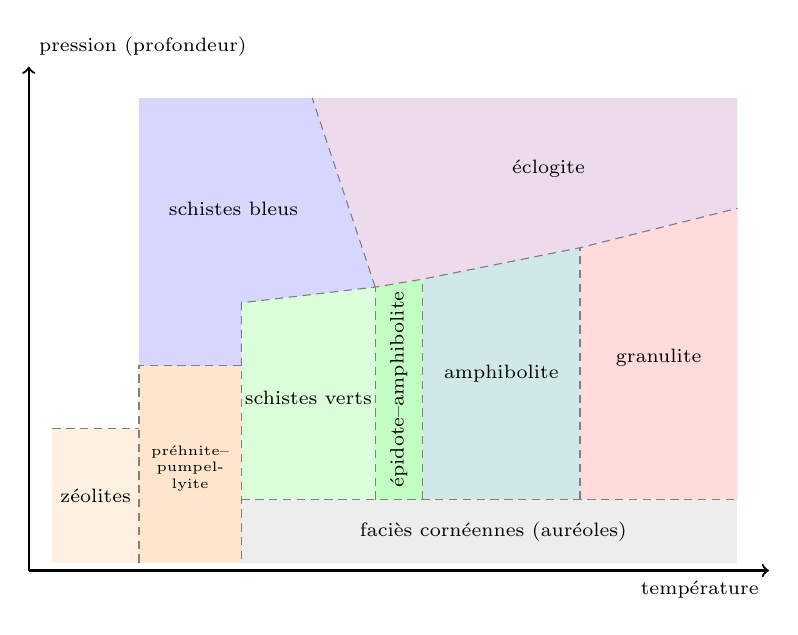
\begin{tikzpicture}[font=\scriptsize, x=1cm, y=1cm]
\draw[->, thick] (0,0) -- (9.4,0) node[below left] {température};
\draw[->, thick] (0,0) -- (0,6.4) node[above right] {pression (profondeur)};
\fill[orange!12] (0.3,0.1) -- (1.4,0.1) -- (1.4,1.8) -- (0.3,1.8) -- cycle;
\fill[orange!20] (1.4,0.1) -- (2.7,0.1) -- (2.7,2.6) -- (1.4,2.6) -- (1.4,1.8) -- cycle;
\fill[green!14] (2.7,0.9) -- (4.4,0.9) -- (4.4,3.6) -- (2.7,3.4) -- cycle;
\fill[green!24] (4.4,0.9) -- (5.0,0.9) -- (5.0,3.7) -- (4.4,3.6) -- cycle;
\fill[teal!18] (5.0,0.9) -- (7.0,0.9) -- (7.0,4.1) -- (5.0,3.7) -- cycle;
\fill[red!14] (7.0,0.9) -- (9.0,0.9) -- (9.0,4.6) -- (7.0,4.1) -- cycle;
\fill[gray!14] (2.7,0.1) -- (9.0,0.1) -- (9.0,0.9) -- (2.7,0.9) -- cycle;
\fill[blue!16] (1.4,2.6) -- (2.7,2.6) -- (2.7,3.4) -- (4.4,3.6) -- (3.6,6.0) -- (1.4,6.0) -- cycle;
\fill[violet!14] (4.4,3.6) -- (5.0,3.7) -- (7.0,4.1) -- (9.0,4.6) -- (9.0,6.0) -- (3.6,6.0) -- cycle;
\draw[gray, densely dashed] (1.4,0.1) -- (1.4,2.6) -- (2.7,2.6) -- (2.7,0.1);
\draw[gray, densely dashed] (0.3,1.8) -- (1.4,1.8);
\draw[gray, densely dashed] (2.7,0.9) -- (9.0,0.9);
\draw[gray, densely dashed] (4.4,0.9) -- (4.4,3.6) (5.0,0.9) -- (5.0,3.7) (7.0,0.9) -- (7.0,4.1);
\draw[gray, densely dashed] (2.7,2.6) -- (2.7,3.4) -- (4.4,3.6) -- (5.0,3.7) -- (7.0,4.1) -- (9.0,4.6);
\draw[gray, densely dashed] (4.4,3.6) -- (3.6,6.0);
\node at (0.85,0.95) {zéolites};
\node[align=center, font=\tiny] at (2.05,1.3) {préhnite--\\pumpel-\\lyite};
\node at (3.55,2.2) {schistes verts};
\node[rotate=90] at (4.7,2.3) {épidote--amphibolite};
\node at (6.0,2.5) {amphibolite};
\node at (8.0,2.7) {granulite};
\node at (5.9,0.5) {faciès cornéennes (auréoles)};
\node at (2.6,4.6) {schistes bleus};
\node at (6.6,5.1) {éclogite};
\end{tikzpicture}
\par\smallskip{\small La \omterm{def:b2:metamorphic-facies:facies}{grille des faciès}, schématique~: l'ordre des faciès du tableau dans le
plan pression--température. Les frontières sont progressives et tracées sans chiffres à dessein~: les
faciès sont définis par leurs assemblages, et les réactions qui les bornent dépendent
de la composition de chaque roche.}
\end{omfigure}
% ledger: scmr:facies, scmr:facies-assemblages

\begin{omfigure}
\centering
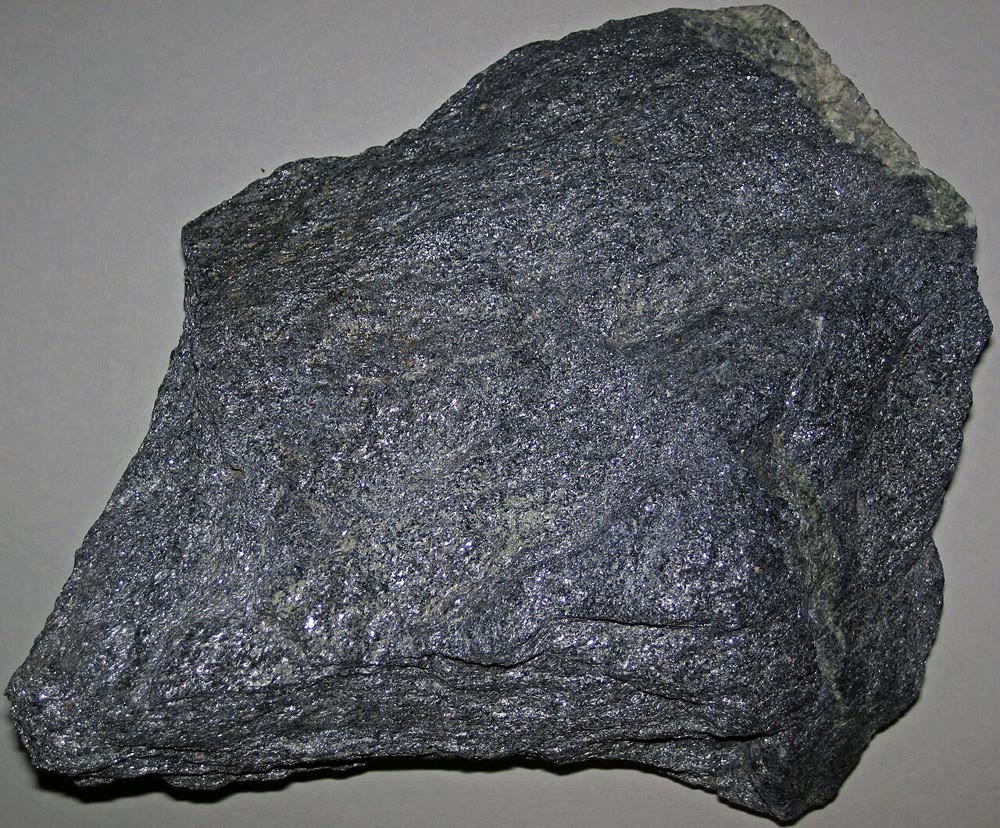
\includegraphics[width=0.27\linewidth]{images/book4/b2-10-blueschist.jpg}\hspace{0.02\linewidth}%
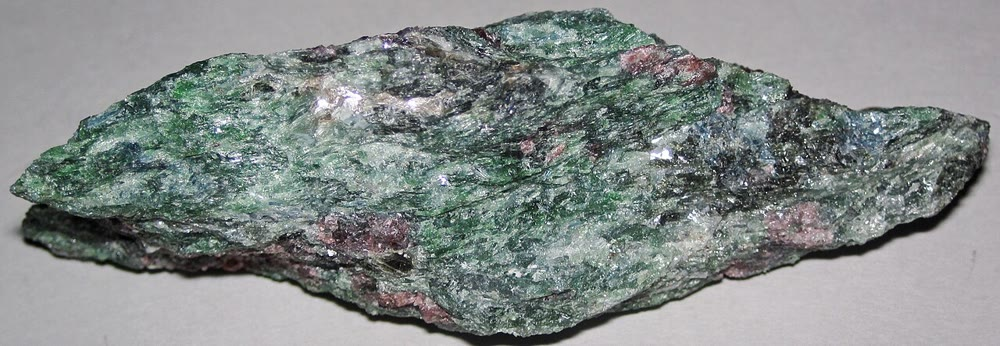
\includegraphics[width=0.69\linewidth]{images/book4/b2-10-eclogite.jpg}
\par\smallskip{\small Deux basaltes métamorphisés. À gauche~: un schiste bleu à lawsonite du
Franciscan Complex de Californie, bleu de glaucophane. À droite~: une éclogite de l'ouest de la
Norvège, à omphacite verte et grenat rouge, avec un peu de quartz, de disthène et de rutile. Photographies
James St.~John, CC BY 2.0.}
\end{omfigure}

Des roches enfouies et chauffées ensemble traversent les faciès dans un ordre régulier, qui
reflète le rapport entre pression et température le long de leur trajet~: élevé dans une zone de subduction,
où se forment les schistes bleus~; intermédiaire dans une chaîne de collision~; bas près d'une intrusion.
\Cref{ch:b2:pt-paths} nomme ces séries et lit de tels trajets à partir des minéraux.
% ledger: scmr:facies

\section{Le protolithe compte}\label{sec:b2:metamorphic-facies:protoliths}

Les faciès sont définis sur les basaltes, mais chaque \omterm{def:b2:metamorphic-facies:metamorphism}{protolithe} enregistre les mêmes conditions dans
ses propres minéraux.

\begin{definition}[Métapélite~; métabasite]\label{def:b2:metamorphic-facies:protoliths}
Une \emph{métapélite}\index{métapélite} est une pélite métamorphisée (roche argileuse), riche en
aluminium et en potassium, dont les assemblages portent micas, chlorite, grenat, staurotide et
les silicates d'alumine. Une \emph{métabasite}\index{métabasite} est un basalte métamorphisé, un gabbro ou
une autre roche mafique, riche en calcium, magnésium et fer, dont les assemblages définissent
les faciès.
\end{definition}

Dans une \omterm{def:b2:metamorphic-facies:protoliths}{métapélite}, les minéraux indicateurs du volume de lycée apparaissent en séquence à mesure que le degré
augmente (chlorite, biotite, grenat, staurotide, disthène, sillimanite), la réaction muscovite + quartz de ce chapitre
fait apparaître la sillimanite et le feldspath potassique à plus haute température encore, et le silicate d'alumine présent
indique de quel côté du point triple la roche est passée. Un calcaire ou une dolomie métamorphisés
deviennent un marbre, de calcite ou de dolomite~; les carbonates impurs, avec silice et argile,
deviennent des roches calco-silicatées dont les réactions de décarbonatation libèrent du dioxyde de carbone~;
un grès quartzeux devient un quartzite, qui ne montre guère que sa taille de grain.
Une \omterm{def:b2:metamorphic-facies:protoliths}{métapélite} de la zone à chlorite et un métabasalte voisin,
à pression et température égales, n'ont rien de comparable,
le second étant une roche verte à actinolite, chlorite, épidote et albite~:
un seul jeu de conditions, deux assemblages.
% ledger: iugs:barrow, day73:ms-qz, scmr:facies-assemblages

\section{Exercices}

\begin{exercise}[$\star$]\label{exo:b2:metamorphic-facies:1}
Nommer le type de \omterm{def:b2:metamorphic-facies:metamorphism}{métamorphisme}~: (a) un calcaire recristallisé en marbre à moins de
\qty{500}{m} d'un granite~; (b) une roche à grain fin et rubanée le long d'une grande faille de décrochement,
ses grains broyés et recristallisés~; (c) un basalte de la croûte océanique dont le
verre s'est transformé en chlorite et en zéolites près d'une dorsale, ses minéraux n'étant que partiellement
remplacés~; (d) des grès volcaniques au fond d'un empilement de \qty{10}{km} d'épaisseur,
recristallisés sans schistosité.
\end{exercise}
% ledger: scmr:types

\begin{exercise}[$\star$]\label{exo:b2:metamorphic-facies:2}
À partir du tableau des silicates d'alumine, calculer $\Delta_r S$, $\Delta_r V$ et la
\omterm{def:b2:metamorphic-facies:clapeyron}{pente de Clapeyron} du disthène $\to$ sillimanite, en \unit{bar/K} et en \unit{MPa/K}. De combien
la pression d'équilibre varie-t-elle sur \qty{100}{\celsius}~?
\end{exercise}
% ledger: rh95:al2sio5

\begin{exercise}[$\star$]\label{exo:b2:metamorphic-facies:3}
À quel faciès appartient chaque métabasalte~? (a) actinolite, albite, chlorite et
épidote~; (b) glaucophane et lawsonite~; (c) hornblende et plagioclase à
\qty{30}{\percent} d'anorthite~; (d) omphacite et grenat, sans plagioclase.
\end{exercise}
% ledger: scmr:facies-assemblages

\begin{exercise}[$\star$]\label{exo:b2:metamorphic-facies:4}
(a) À partir de la masse molaire \qty{162.046}{g.mol^{-1}} et des volumes molaires 44.15, 51.52 et
\qty{49.86}{cm^3.mol^{-1}}, calculer les densités du disthène, de l'andalousite et de la sillimanite.
(b) Laquelle des trois la pression favorise-t-elle, et pourquoi~? (c) Les bases de données minérales donnent 3.61, 3.15 et
\qty{3.24}{g.cm^{-3}}~: pourquoi les cristaux naturels peuvent-ils différer des phases pures~?
\end{exercise}
% ledger: rh95:al2sio5, webmineral:polymorphs

\begin{exercise}[$\star\star$]\label{exo:b2:metamorphic-facies:5}
Pour le disthène $\to$ andalousite, $\Delta_r H = \qty{3.9}{kJ}$, $\Delta_r S =
\qty{8.59}{J.K^{-1}}$, $\Delta_r V = \qty{0.737}{J.bar^{-1}}$. (a) Quel polymorphe est
stable à \qty{25}{\celsius} et \qty{1}{bar}~? (b) À quelle température les deux
coexistent-ils à \qty{1}{bar}~? (c) Calculer la pression d'équilibre à \qty{400}{\celsius} et
la comparer à la valeur expérimentale de \qty{2.54}{kbar}. (d) Pourquoi l'andalousite se trouve-t-elle
néanmoins dans des roches refroidies jusqu'à la surface~?
\end{exercise}
% ledger: rh95:al2sio5, hm93:table11

\begin{exercise}[$\star\star$]\label{exo:b2:metamorphic-facies:6}
Tester l'étape (2) de la méthode. À \qty{1000}{K}, les tables donnent $S_T$ = 285.02 pour le disthène
et 296.44 pour la sillimanite, et $(H_T - H_{298})/T$ = 122.29 et 121.39
(\unit{J.mol^{-1}.K^{-1}}). (a) Calculer $\Delta_r H$, $\Delta_r S$ et $\Delta_r G$ du
passage du disthène $\to$ sillimanite à \qty{1000}{K} et \qty{1}{bar}. (b) Comparer avec les valeurs
constantes de la table. (c) Quel polymorphe est stable là, et quelle est l'erreur de
la méthode simple~?
\end{exercise}
% ledger: rh95:al2sio5-ht, rh95:al2sio5

\begin{exercise}[$\star\star$]\label{exo:b2:metamorphic-facies:7}
La calcite et l'aragonite (\ce{CaCO3}) ont, à \qty{298.15}{K}, $\Delta_f G$ = $-1128.5$ et
$-1127.4$ \unit{kJ.mol^{-1}}, $S$ = 91.7 et 88.0 \unit{J.mol^{-1}.K^{-1}}, $V$ = 36.93
et \qty{34.15}{cm^3.mol^{-1}}, et des enthalpies de formation égales. (a) Trouver la
pression d'équilibre à \qty{25}{\celsius}. (b) Calculer la \omterm{def:b2:metamorphic-facies:clapeyron}{pente de Clapeyron}. (c) Trouver la
pression d'équilibre à \qty{300}{\celsius}. (d) Beaucoup de coquilles sont faites d'aragonite et
vivent à \qty{1}{bar}~: que dit cela~?
\end{exercise}
% ledger: rh95:cc-ar

\begin{exercise}[$\star\star$]\label{exo:b2:metamorphic-facies:8}
Pour l'albite $\to$ jadéite + quartz, les tables donnent $\Delta_r H = \qty{-5.0}{kJ}$,
$\Delta_r S = \qty{-32.4}{J.K^{-1}}$, $\Delta_r V = \qty{-1.698}{J.bar^{-1}}$. (a)
Calculer la \omterm{def:b2:metamorphic-facies:clapeyron}{pente de Clapeyron}. (b) Calculer la pression d'équilibre à \qty{500}{\celsius}.
(c) Les enthalpies de formation de l'albite, de la jadéite et du quartz sont incertaines de 2.6, 3.6
et \qty{1.0}{kJ.mol^{-1}}~; en les combinant comme des erreurs indépendantes, quelle est l'incertitude de cette
pression~? (d) Pourquoi le faciès éclogite est-il dépourvu de plagioclase~?
\end{exercise}
% ledger: rh95:ab-jd-qz, scmr:facies-assemblages

\begin{exercise}[$\star\star$]\label{exo:b2:metamorphic-facies:9}
La muscovite + quartz se décompose à 603, 637 et \qty{662}{\celsius} pour 1, 2 et
\qty{3}{kbar}. (a) Calculer la pente de la droite entre chaque paire de points. (b) Si
l'entropie de réaction varie à peine sur cet intervalle, de quel facteur $\Delta_r V$
a-t-il diminué du premier intervalle au second~? (c) Quelle phase en est responsable~?
\end{exercise}
% ledger: day73:ms-qz

\begin{exercise}[$\star\star\star$]\label{exo:b2:metamorphic-facies:10}
Avec les propriétés constantes de la méthode~: (a) calculer les pressions des trois
réactions à \qty{600}{\celsius}~; (b) montrer qu'à \qty{600}{\celsius} et à la pression du
point disthène $=$ andalousite, la sillimanite est le polymorphe le plus stable, de sorte que ce point de
la droite est métastable~; (c) quel polymorphe est stable à \qty{600}{\celsius} et
\qty{4}{kbar}, et à \qty{600}{\celsius} et \qty{7}{kbar}~?
\end{exercise}
% ledger: rh95:al2sio5

\begin{exercise}[$\star\star\star$]\label{exo:b2:metamorphic-facies:11}
Un schiste renferme ensemble disthène, andalousite et sillimanite, les trois ayant cristallisé à
l'équilibre. (a) Avec le point triple expérimental, $504 \pm \qty{20}{\celsius}$ et
$3.75 \pm \qty{0.25}{kbar}$, et une croûte de densité \qty{2700}{kg.m^{-3}} ($g =
\qty{9.81}{m.s^{-2}}$), à quelle profondeur a-t-il cristallisé~? (b) En prenant \qty{10}{\celsius} à la
surface, quel gradient thermique moyen cela implique-t-il~? (c) Pourquoi de telles roches sont-elles rares~?
\end{exercise}
% ledger: hm93:triple

\begin{exercise}[$\star\star\star$]\label{exo:b2:metamorphic-facies:12}
Deux roches sont enfouies jusqu'à la profondeur $z$, à partir de \qty{10}{\celsius} en surface~: la roche X suit
un gradient de \qty{10}{\celsius.km^{-1}} jusqu'à \qty{30}{km}, sous des roches de densité moyenne
\qty{3000}{kg.m^{-3}}, la roche Y suit un gradient de \qty{30}{\celsius.km^{-1}} jusqu'à \qty{20}{km} sous des roches
de densité moyenne \qty{2800}{kg.m^{-3}}. (a) Calculer $T$ et $P$ à la fin de chaque trajet.
(b) Avec les droites à propriétés constantes (calcite $=$ aragonite~: $P = 13.31\,T$ bar avec $T$
en kelvin~; albite $=$ jadéite + quartz issue de l'\cref{exo:b2:metamorphic-facies:8}~; les silicates d'alumine issus de la
table), laquelle de l'aragonite ou de la calcite, de la jadéite + quartz ou de l'albite, et quel
silicate d'alumine porte chaque roche~? (c) Quel trajet est le plus froid, à haute pression, et dans quel faciès finit chacun~?
\end{exercise}
% ledger: rh95:cc-ar, rh95:ab-jd-qz, rh95:al2sio5

\section{Problème~: construire le point triple}

\begin{problem}[{Problème du week-end --- le diagramme des silicates d'alumine d'après les tables, et jusqu'où
lui faire confiance}]
\label{pb:b2:metamorphic-facies:1}
Utiliser le tableau des silicates d'alumine (\qty{298.15}{K}, \qty{1}{bar}) et la méthode de
ce chapitre, avec $\Delta_r H$, $\Delta_r S$ et $\Delta_r V$ constants~; écrire $T$ en
kelvin, $P$ en bar, et négliger le 1 dans $P - 1$.

\noindent\textbf{Partie I --- Les réactions.}
\begin{enumerate}
\item Calculer $\Delta_r H$, $\Delta_r S$ et $\Delta_r V$ pour le disthène $\to$ andalousite.
\item Faire de même pour le disthène $\to$ sillimanite.
\item Faire de même pour l'andalousite $\to$ sillimanite, et vérifier que chaque grandeur est la
différence des deux premières.
\item Quel polymorphe a la plus grande entropie, lequel le plus petit volume~? De quel côté
de chaque droite chacun se situe-t-il~?
\item Calculer les trois \omterm{def:b2:metamorphic-facies:clapeyron}{pentes de Clapeyron}.
\item Pourquoi la pente de l'andalousite $\to$ sillimanite est-elle négative~?
\end{enumerate}

\noindent\textbf{Partie II --- Où passent les droites.}
\begin{enumerate}[resume]
\item Calculer $\Delta_r G$ des deux premières réactions à \qty{298.15}{K}. Quel
polymorphe est stable à la surface~?
\item À quelle température (en \unit{\celsius}) chaque réaction atteint-elle l'équilibre à
\qty{1}{bar}~?
\item Parmi les trois températures de la question~8, lesquelles sont des équilibres stables et lesquelles
métastables~? (Utiliser l'ordre des trois à \qty{1}{bar}.)
\item Calculer la pression de l'équilibre disthène $=$ andalousite à \qty{400}{\celsius}~; les
expériences donnent \qty{2.54}{kbar}.
\item Calculer la pression de l'équilibre disthène $=$ sillimanite à \qty{700}{\celsius}~; les
expériences donnent \qty{7.86}{kbar}.
\item Esquisser les trois droites entre 200 et \qty{900}{\celsius}.
\end{enumerate}

\noindent\textbf{Partie III --- Le point triple.}
\begin{enumerate}[resume]
\item Écrire les deux premières droites sous la forme $P = a_i T - b_i$~; donner $a_1$, $b_1$, $a_2$, $b_2$.
\item Déterminer la température de leur intersection.
\item Calculer sa pression.
\item Vérifier que l'équilibre andalousite $=$ sillimanite passe par ce point.
\item Comparer aux valeurs expérimentales $504 \pm \qty{20}{\celsius}$ et $3.75 \pm
\qty{0.25}{kbar}$.
\item En tenant compte de la dépendance en température des tables, le point triple se déplace à
\qty{536}{\celsius} et \qty{4.20}{kbar}. Le raffinement l'a-t-il rapproché de
l'expérience~? Qu'est-ce que cela suggère quant à la principale source d'erreur~?
\end{enumerate}

\noindent\textbf{Partie IV --- Jusqu'où lui faire confiance.}
\begin{enumerate}[resume]
\item Augmenter l'enthalpie de formation de l'andalousite de \qty{1}{kJ}. De combien la droite
disthène $=$ andalousite se déplace-t-elle en pression, à température fixée~?
\item De combien le point triple se déplace-t-il en température~?
\item Faire de même pour une hausse de \qty{1}{kJ} de l'enthalpie de la sillimanite.
\item Chaque enthalpie est incertaine de \qty{2.0}{kJ}. Quelle plage de températures de point triple
les seules données calorimétriques permettent-elles~?
\item Comment, dès lors, des tables thermodynamiques peuvent-elles reproduire le diagramme expérimental à
\qty{30}{\celsius} près~?
\item Donner la température du point triple calculée dans la partie III, arrondie au
degré près~: le nombre clé de ce problème.
\end{enumerate}
\end{problem}
% ledger: rh95:al2sio5, rh95:al2sio5-ht, hm93:triple, hm93:table11, hm93:adjusted
